\label{sec:arbitrage}
\begin{figure*}[!ht]
    \centering
    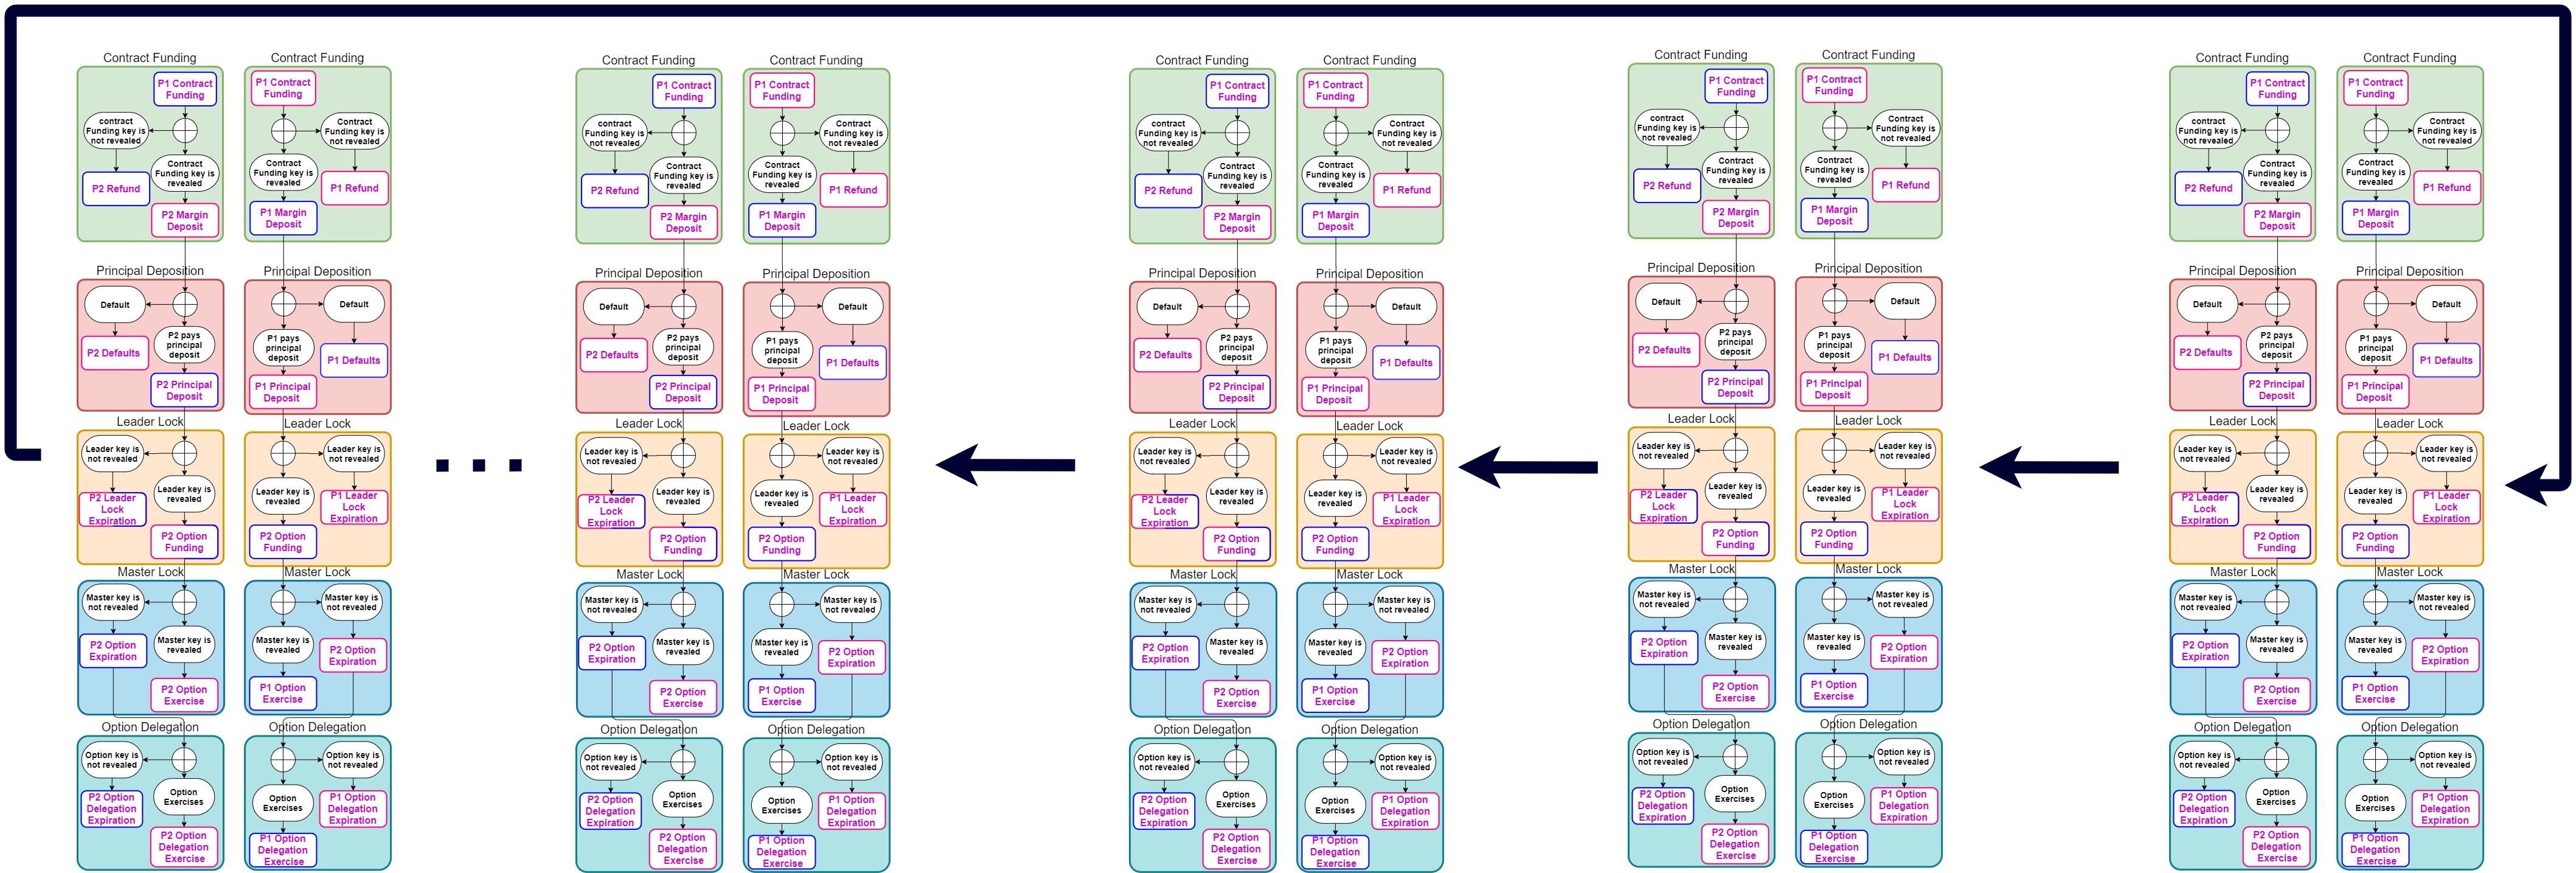
\includegraphics[width=\textwidth]{figures/looped arb.png}
    \caption{General form of the looped Arbitrage, composed of several instances of meta swaption.}
    \label{fig:meta_arb}
\end{figure*}

In this section we are going to elaborate on the term of arbitrage by redefining it in swaption market in the following way:
An arbitrage in the swaption market is an opportunity when a party, named exploiter, can exercise a chain of swaptions simultaneously, beginning from the exploiter's asset and also ending in the same asset, and profits by gaining more assets than the start point. Fig~\ref{fig:meta_arb} shows the general form of an arbitrage made up of several instances of \MetaSwaption forming a loop.

% \begin{definition}{\it Arbitrage Owner}
% In an arbitrage, the one who buys all the swaptions is called the Arbitrage Owner. In our examples she mostly is Alice. The Arbitrage Owner is also called the \Atwo Key Holder interchangeably.
% \end{definition}

We introduce four different types of arbitrages that are possible by adoption of our \MetaSwaption as their building blocks:
\begin{itemize}
    \item \textbf{Early deposition} arbitrage
    \item \textbf{Late deposition} arbitrage
    \item \textbf{Margin-free} arbitrage
    \item \textbf{Bonded} arbitrage
\end{itemize}


For further analysis, we give an example of arbitrage use cases. Alice, the exploiter whose initial asset is ACoin, is going to form an arbitrage making a chain of swaptions between Bob, Carol, Dave and Erin that take place concurrently. In section~\ref{sec:tangle} we will explain the procedure of signing contracts for each party in details but first we discuss about the general overview of our execution processes. For convenient reason, we index each swaption by order, \ie indexes of swaptions between Alice and Bob, and Alice and Carol, and Alice and Dave and Alice and Erin are respectively one to four.

Using the normal form of arbitrage shown in Fig.~\ref{fig:sep-arb}, the exploiter has to pay margin in every single swaption besides generating lots of transactions and thus, transaction fees. To solve this and to exercise the swaptions concurrently, we use the overlapping technique which changes the structure of our arbitrage model to Fig.~\ref{fig:overlap-arb}.

The overlapping technique is the action of extending the output's required signatures of all transactions to other parties in order to make additional guarantee.

\begin{figure}[htp]
    \caption{Arbitrage with and without overlapping technique}
    \subfloat[Arbitrage architecture using a loop of swaptions]{
    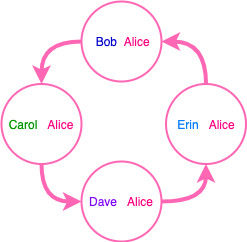
\includegraphics[width=0.45\textwidth]{figures/arb-sep.png}
    \label{fig:sep-arb}
  }~
  \subfloat[Arbitrage architecture using overlapping technique]{
  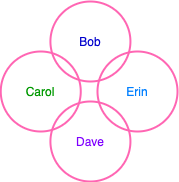
\includegraphics[width=0.45\textwidth]{figures/arb-overlap.png}
  \label{fig:overlap-arb}
  }
\end{figure}


% \begin{definition}{\it Genesis swaption}
% In an arbitrage, the swaption in which \Atwo key holder and \keyone key holder are faced together is called the Genesis Swaption. This swaption is supposed to be the first one processed in an arbitrage. 
% \end{definition}

%\subsection{Model}
% \subsection{Lined Arbitrage}
% \ahC{Are these lines in the good position?}

\subsection{Early Deposition Arbitrage}
\label{sec:line_arb}

Consider the following variation of our main example. Alice already has an amount of ACoin equal to the needed principal. First of all, she starts a swaption with Bob. After Bob deposits his principal, Alice can use his BCoins on her later swaption contracts. Then she trades these locked BCoins with Carol's CCoins, and these CCoins with Dave's DCoins and finally trades these DCoins with Erin's ACoins. According to the definition of arbitrage, now she has more ACoins than she primarily had. Since Alice primarily has enough ACoins, she only uses early deposition swpations. She technically can use a late deposition swaption for the first swaption, but since in that case she has to pay larger premium, it is not rational.
She also uses the swaption overlapping to transfer her assets between different swaption contracts. 
In Fig~\ref{fig:line_arb} this technique is shown. All parties share all transaction before any thing gets broadcast. After that, the procedure goes on as follows:

\begin{figure*}
    \centering
    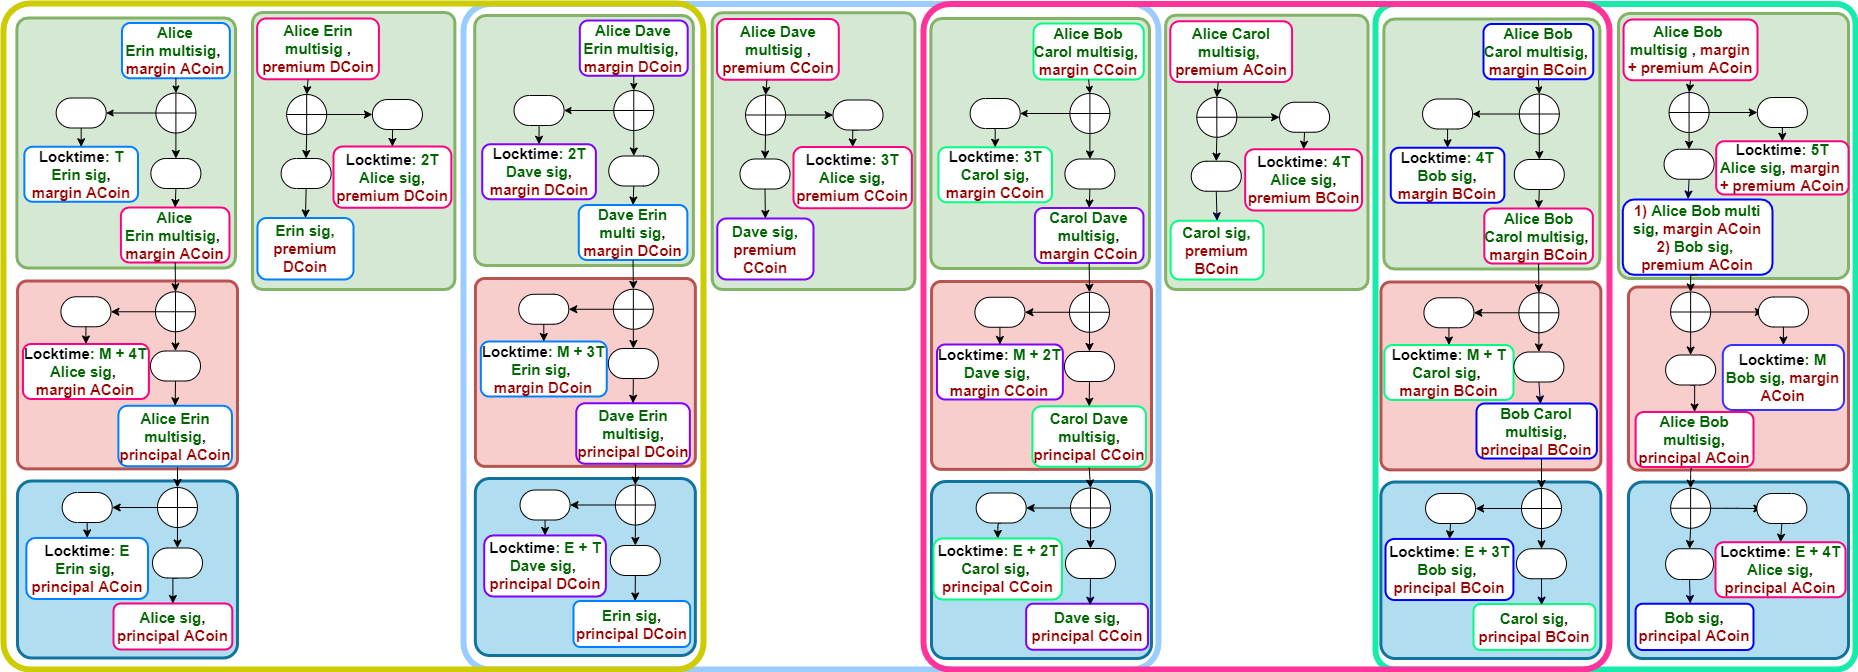
\includegraphics[width=\textwidth]{figures/arbitrage1-fateme.png}
    \caption{Example of an arbitrage, where Alice owns all ACoins primarily needed. On each transaction, signatures, output amount, and locktimes are specified. Pink-bordered transactions are broadcast by Alice, blue-bordered ones by Bob, green-bordered by Carol, purple-bordered by Dave and cyan-bordered by Erin. If there is a line between two transactions, then the source transaction is considered to be an input of the destination transaction.}
    \label{fig:line_arb}
\end{figure*}

\begin{itemize}
    \item \textbf{Contract funding}: Alice starts her contract with other parties simultaneously, by sharing the funding transaction with them. Then she decides whether to reveal \Aone key or not. If she does, all the swaptions go to the next stage. The locktimes are set descending from swaption number one to four, so that Alice can not cheat. In fact, Alice has to reveal \Aone before $T$, the minimum locktime among all swaptions, since otherwise at least one of them has expired and the entire arbitrage is not plausible any more. Note that if any of the funding stages fail, the entire arbitrage fails.
    
    \item \textbf{Principal deposition}: In this stage, every one has to deposit their principal. All swaptions are early deposition swaptions, so all the locktimes are ascending from swaption number one to four. Possible scenarios: 
    \begin{itemize}
        \item One of the parties defaults. In this case, all parties after the defaulter also default. Hence, the first defaulter looses his margin and all the other parties transfer their margin with the next party in the swaption with the next index and the last party transfers her margin to Alice.
        \item All parties deposit their principal and go to the next stage.
        
    \end{itemize}
    
    % \item \textbf{Leader Lock}:The locktimes in the first swaption are ascending and in the rest of swaptions are descending. The reason is that in the first one Bob holds the \keyone key and in other ones Alice holds it. Note that Bob has the M + P + 3T locktime but in fact he has to reveal \keyone key before M + P, because otherwise Alice defaults and Bob loses his margin. parties take back their own money. By arranging timelocks in this way, no portion of parties can cheat on others by cooperating. Possible scenarios:
    
    % \begin{itemize}
    %     \item Bob defaults. he looses one of his margins as discussed in {\it Late Deposition} swaption, while other
    %     \item Bob reveals \keyone key by broadcasting Alice's option funding transaction. Then Alice broadcasts the Erin's Option Funding transaction, and other opponents do the same respectively. And we go to next stage. If any of them does not do this, the only one who looses money is that party.
    % \end{itemize}
    % \ahC{is it clear and okay or not? We can mention that all of the swaptions in the point of view of other opponent than Alice is just like an instance of Meta Swaption, accordingly no body can cheat by cooperation on others}
    
    \item \textbf{Option funding}: It is time for Alice to use her option. She reveals \Atwo key for Erin, then each party reveals it for the previous one in order. Therefore, the locktimes are descending in all swaptions from swaption number one to four.
\end{itemize}

\subsection{Late Deposition Arbitrage}
\label{sec:margined_arb}
% \subsubsection{Margined Arbitrage}
Now, consider the case that Alice does not own enough ACoin to start such a procedure. She has to pay ACoin to Bob using a portion of ACoins she gets from Erin. This would only be possible if she had the ability to spend Bob's BCoins and do all the tradings with it and finally deposit the ACoins taken form Erin to the first swaption. To do so, she can use the late deposition swaption as the first swaption. We call it the late deposition arbitrage. Fig.~\ref{fig:margined_arb} depicts such an arbitrage. There are four swaptions, and Alice pays only premium in all of them. She also has to deposit margin in the first swaption. Alice's margin is only there to prevent her from cheating due to the cyclic locktimes on the funding stages (in the next section we will briefly explain this problem and our proposed solution). Therefore, there are five margins and four swaptions. The first swaption to start is the same as the last swaption to finish and it is actually between Erin and Bob (swaption number one). The five phases of late deposition arbitrage are: 

\begin{figure*}
    \centering
    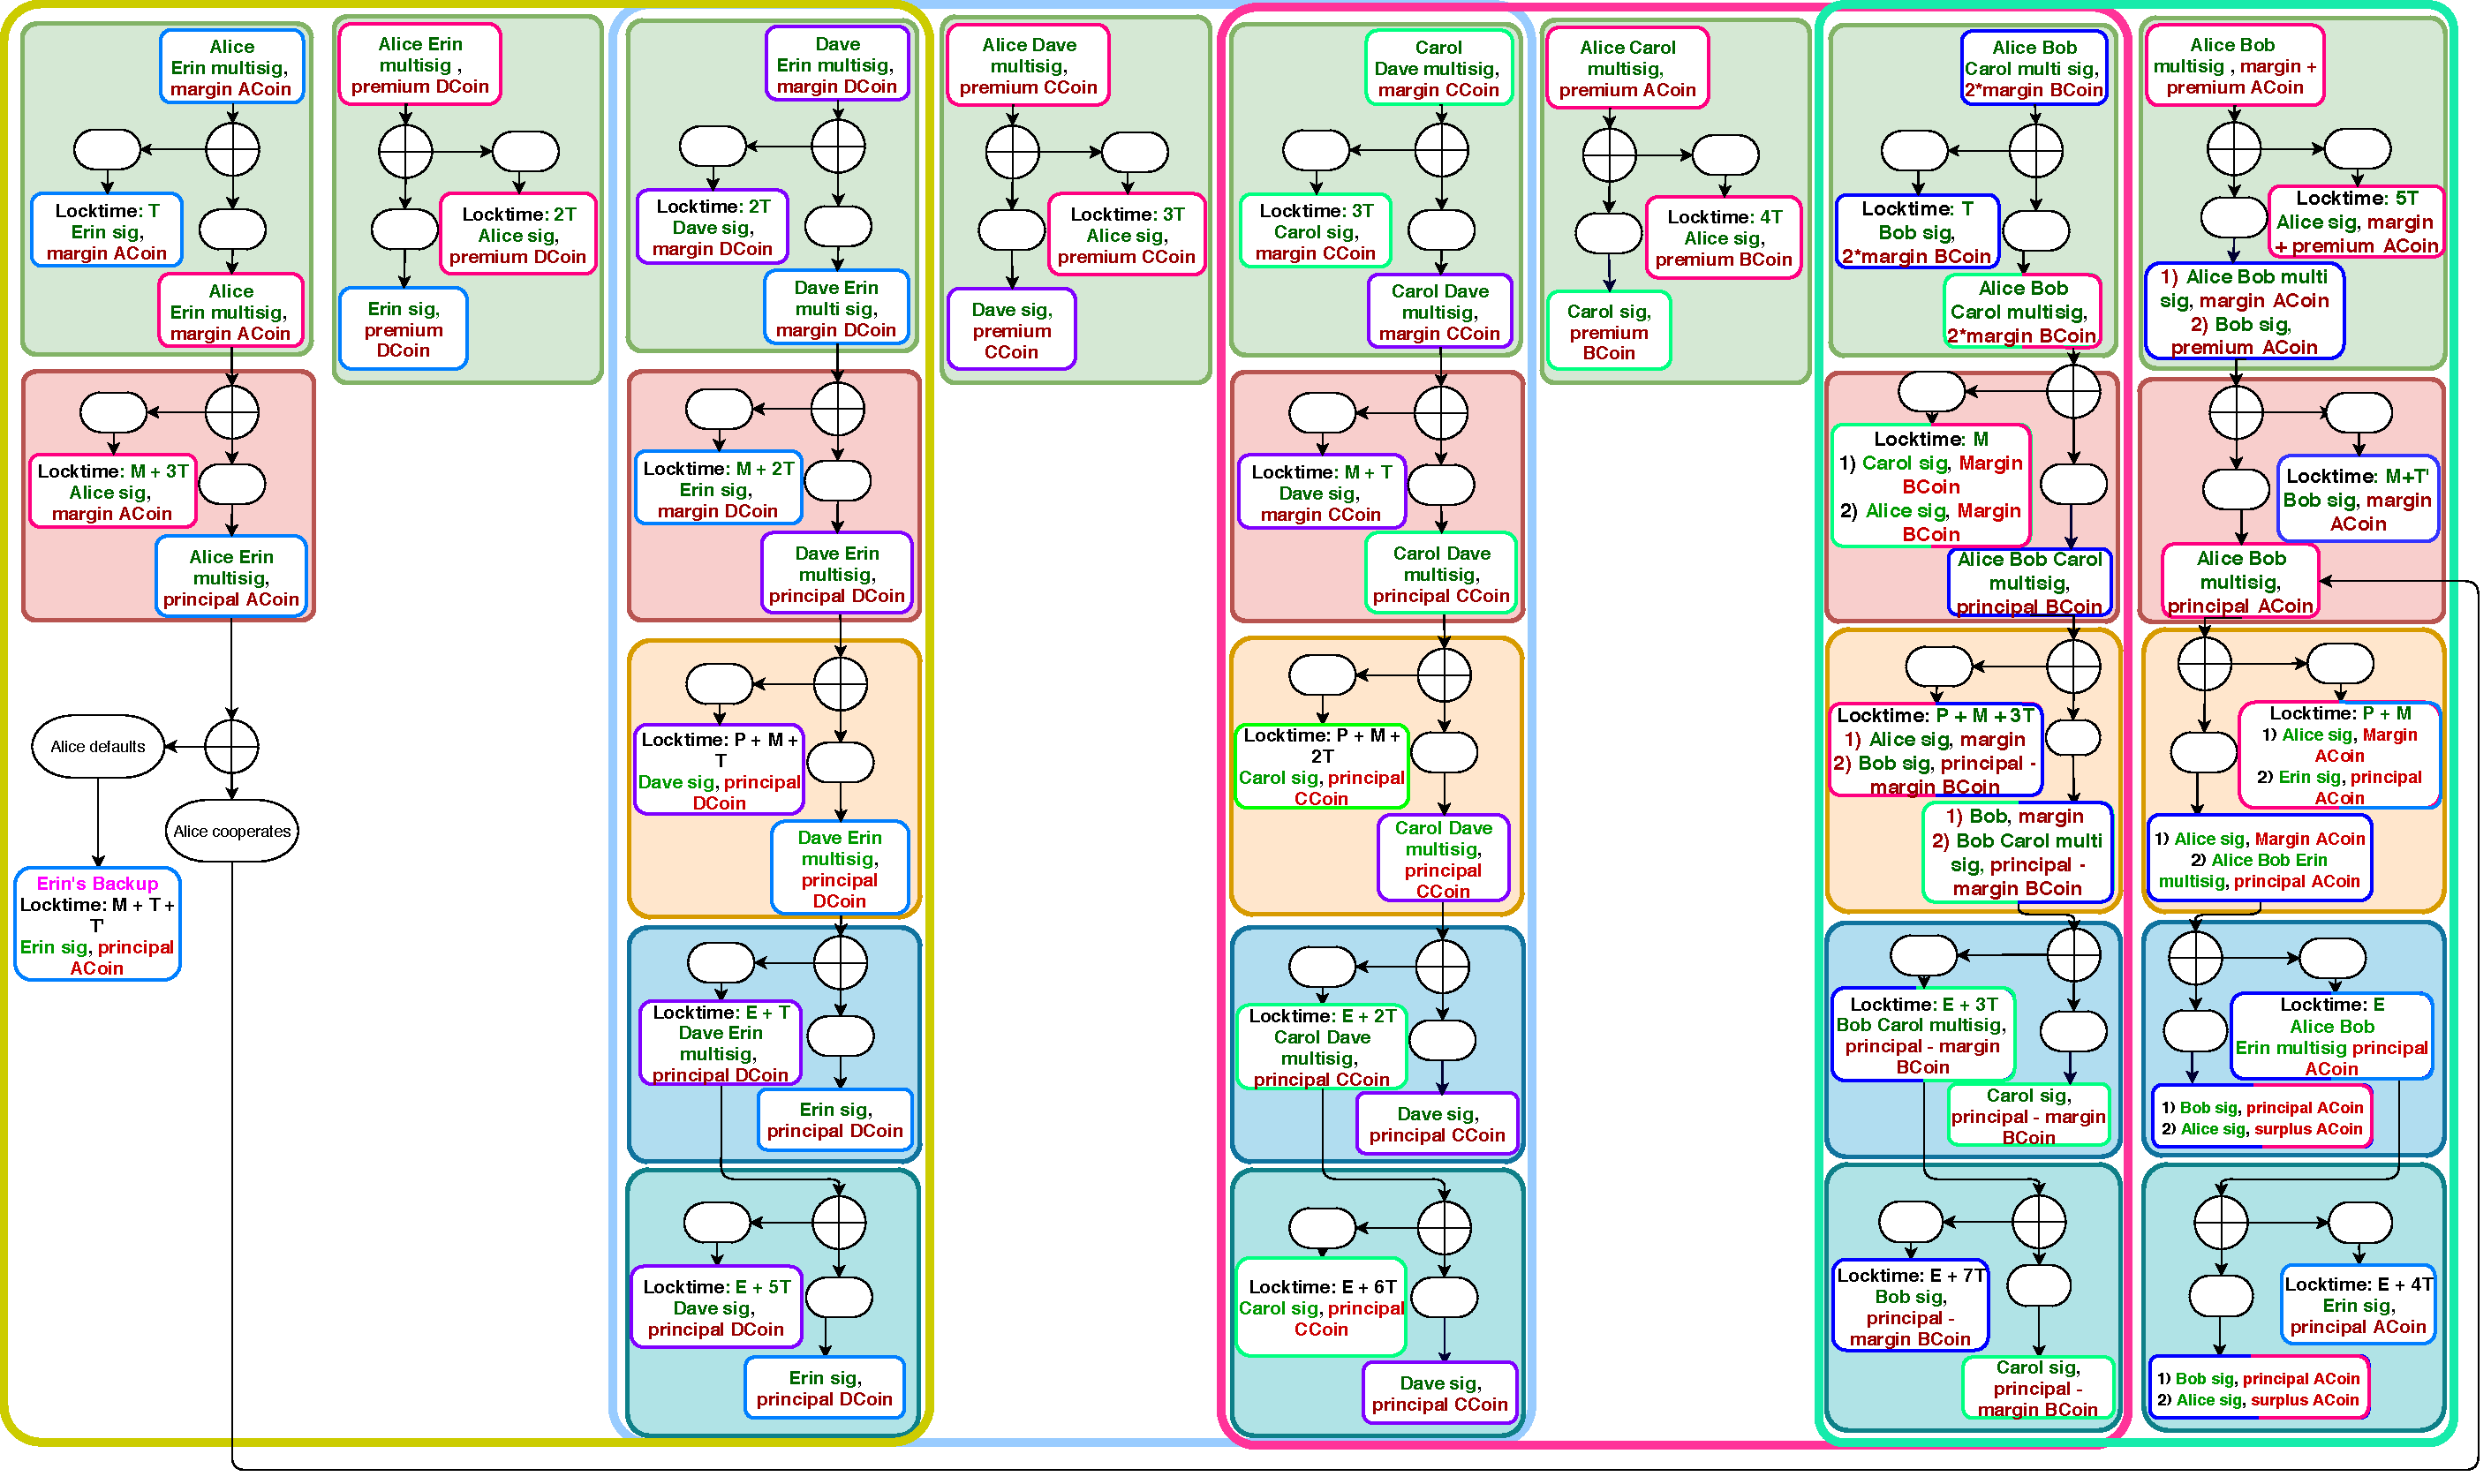
\includegraphics[width=\textwidth]{figures/arbitrage-late.pdf}
    \caption{The schematic for late deposition arbitrage. The transactions with two border colors, can be broadcasted with both corresponding parties.}
    \label{fig:margined_arb}
\end{figure*}


\begin{itemize}
    \item \textbf{Contract Funding}: Similar to the early deposition arbitrage, every one has exchanged funding and refund transactions. Three types of these stages:
    \begin{itemize}
        \item Alice's first funding includes margin + premium.
        \item Other fundings of Alice only include premium.
        \item Bob's funding includes margin and an amount of guarantee. Here the amount of guarantee is equal to the margin, so Bob's funding is worth twice other parties margins.
        \item Other parties fundings include only margin.
    \end{itemize}
    Alice reveals the \Aone key by broadcasting Erin's margin deposit transaction. Then, Erin broadcasts Dave's margin deposit transaction and everyone broadcasts the margin deposit transaction of their previous party. No one has the incentive not to broadcast this transaction since if she does not, she is the only one who goes through a loss. When all the margin deposit transactions are broadcast, the arbitrage proceeds to the next stage.
    
    \item \textbf{Principal deposition}: All swaptions except for the first one are early deposition, so the locktimes of principal deposition on these swaptions are ascending from swaption number two to four. On the other hand, the first swaption is late deposition, so Alice's locktime has to be greater than Bob's. Alice's principal is in fact a portion of the principal that Erin deposits. Similar to the early deposition arbitrage, if any one defaults in this stage, and does not deposit his principal, the faulty party loses his margin (except for when it is Alice that exchanges her margin with Bob's) and other parties margins are exchanged with their previous party. As mentioned earlier, the first swaption is in fact between Erin and Bob, but Alice also puts margin to this swaption. The principal deposition of Erin is an any-one-can-pay transaction. The amount of $M+T'$ needs to be greater than $M+3T$, hence if Erin defaults, Alice can default too. If Erin does not default and broadcasts her principal deposition transaction, Alice takes its output as an input to the principal deposition of the first swaption. We have given Erin a chance that if Alice does not do so, she can take her principal back and of course since Alice has defaulted, she exchanges her margin with Bob's. If everyone deposits their principal, we go to the next stage.
    % \ahC{Revise the entire paragraph}
    \item \textbf{Leader lock}: Alice is waiting for Bob to reveal the \keyone key by broadcasting the Erin's option funding transaction on first swaption. If Bob does so, Erin broadcasts Dave's option funding transaction and every other party broadcasts the previous party's option funding transaction respectively. Locktime for Alice is the shortest and increased from swaption number four to two and for Bob is the longest. Bob's option funding transaction can be broadcasted by both Carol and Bob. Otherwise, other parties can collude and cheat on Bob using the following attack: Bob reveals the \keyone key and others do not broadcast the Bob's option funding and take Bob's margin. Hence, when Bob can broadcast his own option funding, there would not be any problem of this kind. 
    
    Thus, if Bob reveals the key, every other party goes to the next stage. If Bob does not reveal, he loses his margin. If Bob reveals the \keyone key after $P + M$, Alice will take back her margin and immediately reveal the \Atwo key which results in taking Bob's money in both swaptions, thus discouraging Bob from delaying in exposure. 

    \item \textbf{Option funding}: This is the time for Alice to use her option. She can reveal the \Atwo key by broadcasting the Erin's option exercise. She takes her surplus and Bob gets his ACoins. She has to reveal it within $E$ locktime. Since in all swpations the buyer party,
    \ie right-hand side party, is in charge of revealing the \Atwo key, the locktimes have to be descending. This means the locktime of the Erin's option expiration transaction has to be both longer and shorter than the Bob's option expiration. This is obviously impossible. Hence, we set the locktimes so that Carol's locktime is longer than Alice's, which makes it possible for Carol and Alice to cheat on Bob, but we solve this problem using the delegation stage. Now, if Alice exercises her option until $E$ locktime, then every party can take their new coins. If Alice does not exercise until $E$, her option is delegated to Bob.
    
    \item \textbf{Option delegation}: If Alice has not exercised until $E$, Bob broadcasts the Erin's option expiration and Bob's option expiration transactions and all other parties do the same (since it is their only chance to get their coins). The arbitrage is now in the delegation stage. Bob has the option and everyone is waiting for him. If he decides to exercise, everyone gets their new coins, otherwise everyone gets their former coins. The locktimes are descending for all swaptions except for the first one which is ascending (like last stages), since now Bob is the key holder of this stage and he is in charge of revealing the \Delegation key. 
    % \fatemeC{The most important consideration is that if Alice has decided not to exercise her option, Bob would also not exercise. Since if it was not beneficial for Alice it would not be beneficial for Bob neither. the reason is that the coins that Alice gets are the same as Bob gets, so if one has lost its value the other one has lost too.(why the hell????)}
 
\end{itemize}
\begin{figure*}
    \centering
    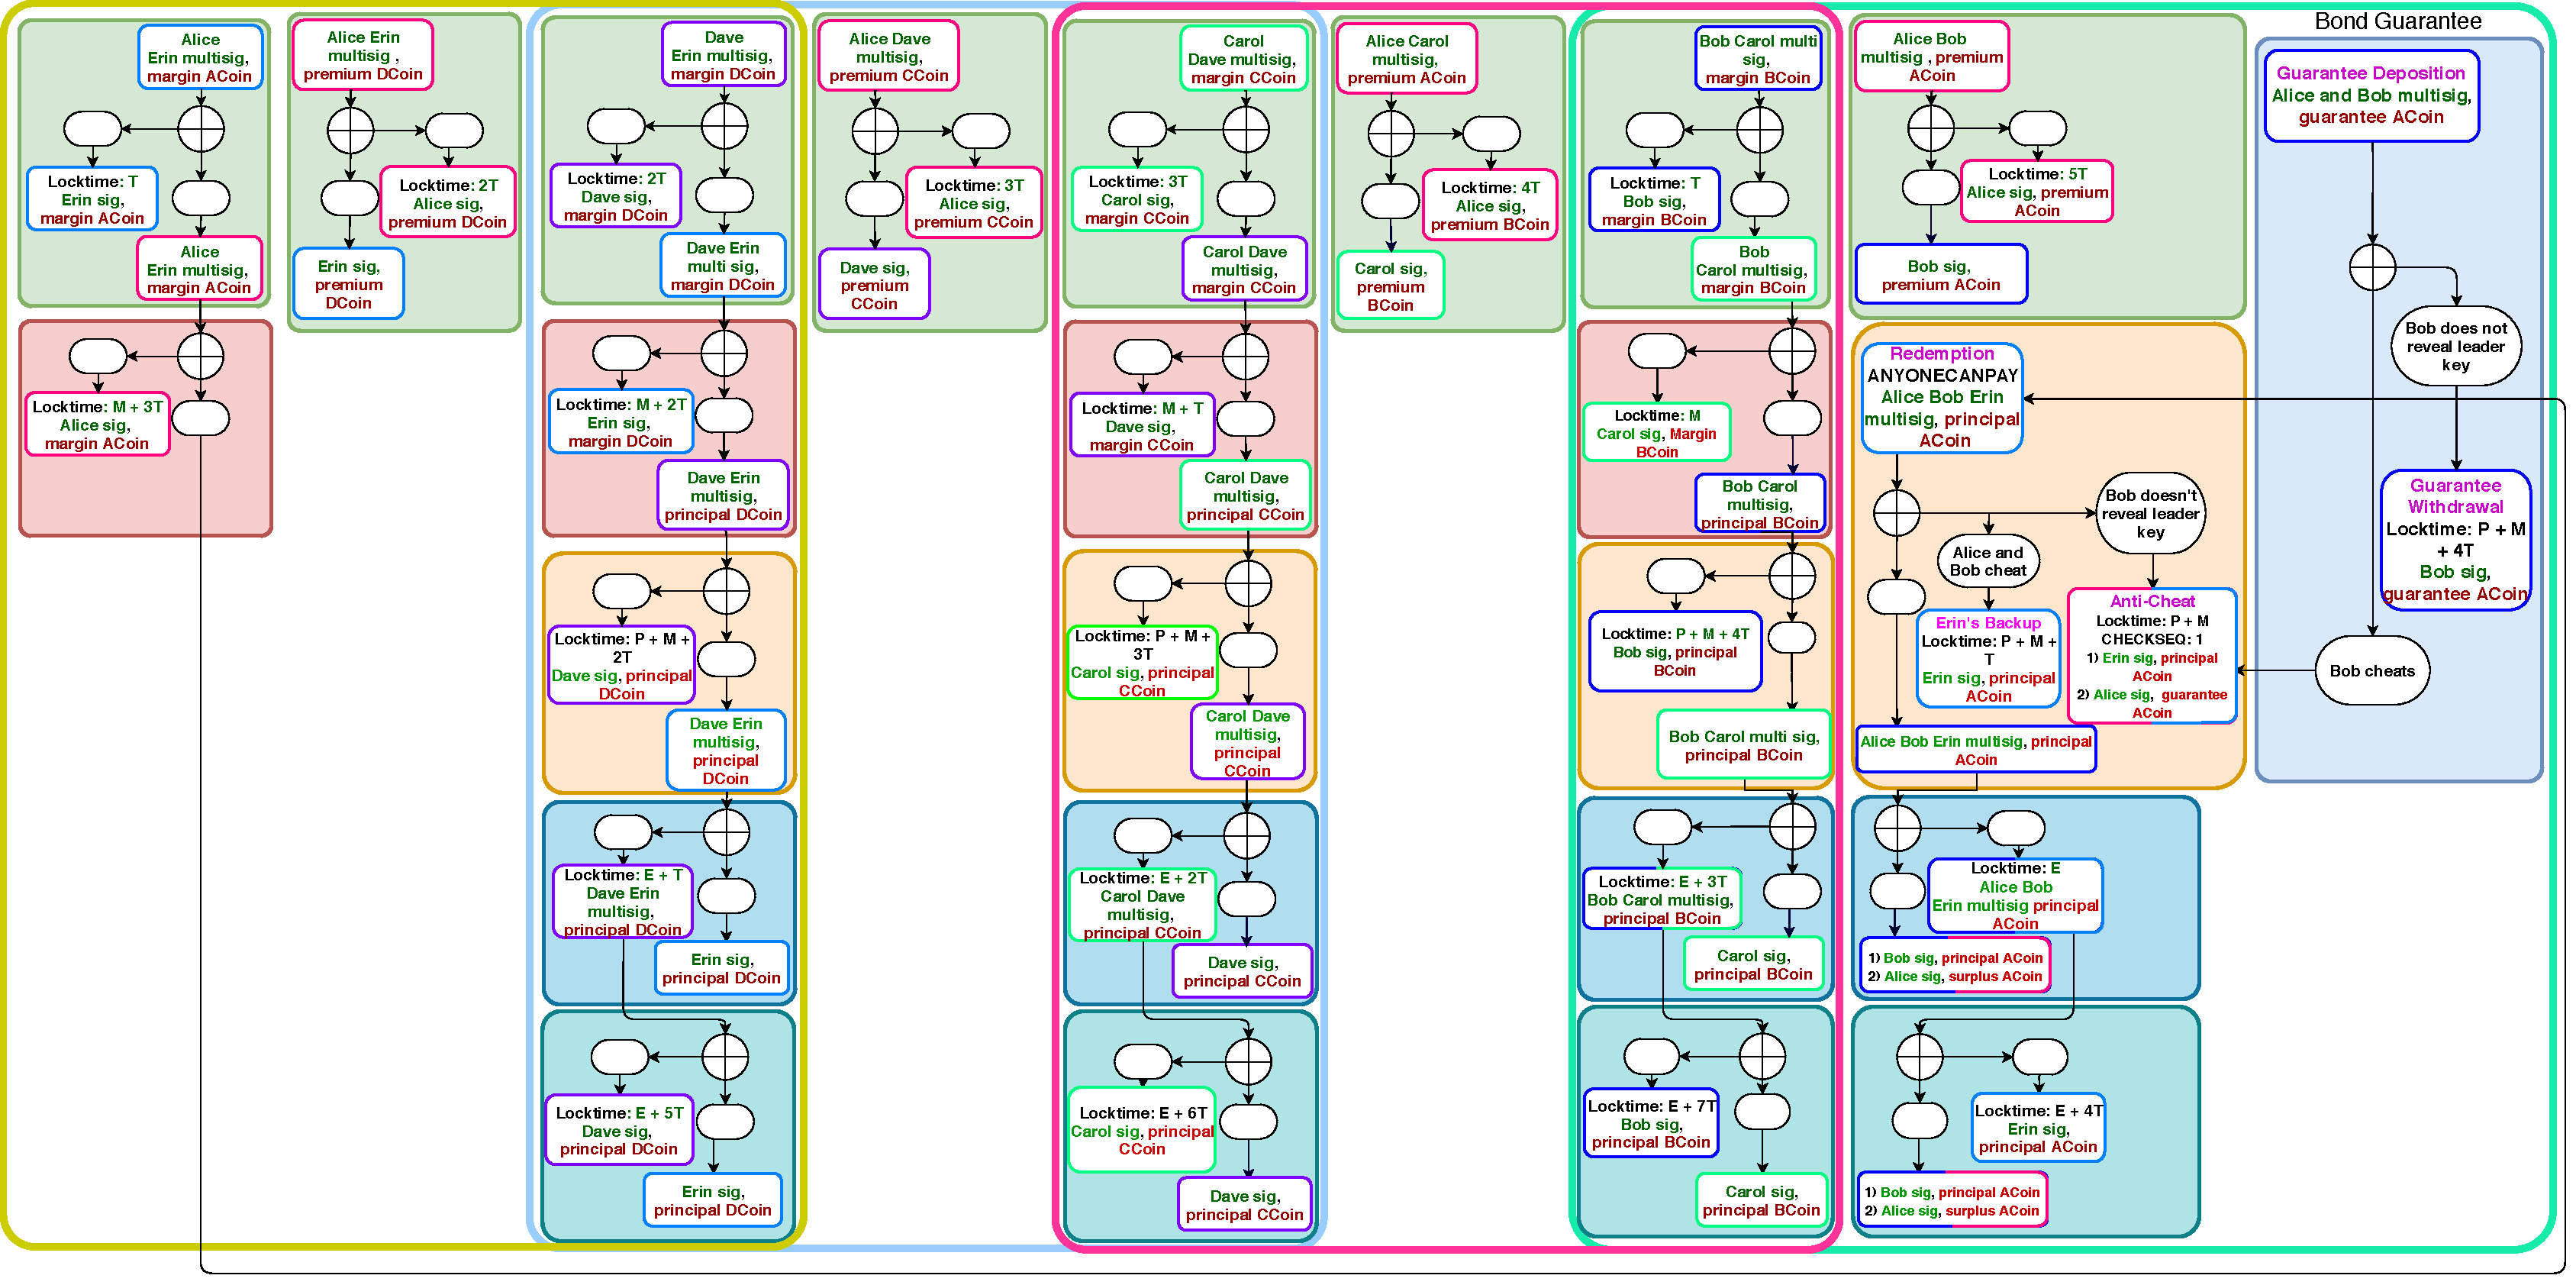
\includegraphics[width=\textwidth]{figures/arbitrage-bonded.pdf}
    \caption{The bonded arbitrage using ABCD.}
    \label{fig:abcd-arb}
\end{figure*}

\subsection{Margin-Free Arbitrage}
%\vspace{-1mm} 
Next, we are going to study the case in which Alice does not have enough ACoin for margin deposition in her swaption with Bob but still she can afford the minimal amount of ACoin as guarantee besides all the premiums. Using the margin-free swaption mentioned in previous section, an arbitrage can be built and exploited satisfying our need. Before all, we have to analyse the amount of guarantee in a margin-free swaption. If this type of swaption is used lonely without further contracts, the minimum valuable amount is enough for the amount of guarantee (even if it is less than premium). However, to use it alongside other contracts, \eg~as the first swaption in an arbitrage setting, Alice needs to set the guarantee value of Bob more than the summation of all the premiums which she wants to spend in her later contracts. Otherwise, Bob is incentivized to pretend himself as the other parties in later contracts, \eg~in our example Carol or Dave or Erin, and cheats on Alice by stealing Alice's premiums in the later swaptions by not exposing the \keyone key and loosing his guarantee. Note that if Bob acts honestly, the guarantees in both sides will be exchanged. In fact, assume the amount of margin is worth $m$ times more than the amount of premium. The margin-free swaption can be used, if the number of parallel swaptions, is less than $m$. Otherwise, it is better to use a late deposition swaption instead. We do not include the figure for margin-free arbitrage, however, it is simply derivable from previous arguments.

\subsection{Bonded Arbitrage}
For final case, we suppose that Alice even does not have enough money for guarantee needs in a margin-free swaption. Alice still can make an arbitrage using the ABCD component devised in previous works, as her first swaption \cite{tefagh2020atomic}. In this way, she does not need more money than the premiums for her arbitrage. We call this type of arbitrage, the bonded arbitrage, since the arbitrage exploiter bonds her initial asset in the first place. The bonded arbitrage is shown in Fig.~\ref{fig:abcd-arb}.
% \ahC{The figure is ABD, we need an ABCD one}

\begin{table*}[]
    \centering
    \begin{tabular}{|c|c|c|c|}
    \hline
        {\normalsize Stage} & {\normalsize LT in column $1$} & {\normalsize LT in column $2i$} & {\normalsize column $2i + 1$}\\
        \hline
        
        {\normalsize Contract Funding} &
        {\normalsize $(N + 1)T$} &
        {\normalsize $(N - i + 1)T$} &
        {\normalsize $(N - i + 1)T$} \\
        
        {\normalsize Principal Deposition} &
        {\normalsize $M + T'$} &
        {\normalsize $M + (N - i)T$} & - \\
        
        {\normalsize Leader Lock} & {\normalsize $P + M$} &
        {\normalsize $P + M + iT$} & - \\
        
        {\normalsize Option Contract} & 
        {\normalsize $E$} &
        {\normalsize $E + (N - i)T$} & - \\
        
        {\normalsize Option Delegation} & 
        {\normalsize $E + NT$} & 
        {\normalsize $E + (2N - i)T$} & - \\
        \hline
    \end{tabular}
    \caption{Locktimes for general case in an arbitrage. Each column in the table shows one column in the arbitrage.}
    \label{tab:arb}
\end{table*}

Now, consider the general case for the arbitrage when there are $N$ swaptions.
Table \ref{tab:arb} shows locktimes for each stage in a general arbitrage. Each column in the table shows one column in the arbitrage. Moreover, for simplicity we put locktimes so that different stages do not have overlap in time. In some cases overlapping stages can cause trouble. Two examples are: 

\begin{itemize}
    \item $M$ has to be larger than $(N + 1)T$. Otherwise, Alice and Carol can broadcast the Bob defaults transaction and then broadcast the Alice's refund and take Bob's margins.
    
    \item In the third stage, $P + (N - 1)T$ has to be greater than $T'$. Otherwise, Alice can wait untill $P + M + (N - 1)T$ not depositing principal, then Bob has to broadcast the Bob's leader key expiration and then Alice will deposit and then broadcast the Alice's leader key expiration. So, she takes Bob's margin without loosing anything but premium.
\end{itemize}

Note that Alice in fact has $E$ time to use her option. Then Bob takes the option, so we can say that Alice does not have any option but it is not true for two reasons: 1) Arbitrages are always zero-risk. 2) If she deposits her principal it means that all the parties have cooperated (if one does not, she does not deposit principal and does not lose anything, just the margins are exchanged which is inevitable). When all parties have cooperated and arbitrage is zero-risk every thing is fine so why would Alice not exercise?

Note that in such cases Alice is always going to use her option, so Alice is not in fact delegating her option to Bob, but by having the delegation stage, she only assures Bob that he would not be cheated.
%\ahC{koja tozih dadim ke delegation mitone bejaie oon method e maskhareie Atomic Cross-chain Swap estefade beshe?}

% \ahC{Time Elapsed Experiment.}\\
% \ahC{Reconstruction impossibility}\\
% \fatemeC{Is it reasonable to remove Option parts from Arbitrage. Arbitrages have absolute benefit in a short time, so the option is not needed to be given to Alice. However she can have it by adding the rest of the transactions.}\\